\section{实验评估}

\subsection{纹理质量定量比较}

\subsubsection{实验设置}

本节对完整两阶段流程进行定量评估，
即以单张参考图像为输入，
经多视角扩散模型生成多视角图像后，
再由微调的 Trellis.2 完成三维纹理生成。
测试集由 64 个艺术家创作的三维模型构成，
每个模型配有对应的参考图像。

评估流程如下：对每个测试模型，以参考图像和裸网格为输入，
生成带纹理的三维模型，
随后对生成模型进行多视角渲染以获取评估图像。
具体而言，渲染采用透视投影，沿水平方向均匀采样 120 个视角，
渲染分辨率为 $512 \times 512$，
所有渲染图像均合成于黑色背景以消除背景干扰。
最终将全部渲染结果与参考图像进行逐指标比对，
同时单独统计正面视角的指标以评估正面纹理保真度。
本文采用以下四个指标进行评估：

\begin{itemize}
    \item \textbf{LPIPS}（Learned Perceptual Image Patch Similarity）\cite{zhang2018unreasonable}：
    基于深度特征的感知相似度距离，衡量生成纹理与参考图像在感知层面的整体一致性，越低越好。
    \item \textbf{Front LPIPS}：仅取正面视角渲染图与参考图像计算 LPIPS，
    重点衡量模型在正面（即参考图像直接可见区域）的纹理保真度。
    \item \textbf{FID}（Fréchet Inception Distance）\cite{heusel2017gans}：
    衡量生成图像分布与参考图像分布之间的距离，反映整体生成质量，越低越好。
    \item \textbf{CMMD}（CLIP Maximum Mean Discrepancy）\cite{jayasumana2024rethinking}：
    基于 CLIP 特征的分布距离度量，对语义层面的分布差异更为敏感，越低越好。
\end{itemize}

基线方法包括：Hunyuan 2.0\cite{zhao2025hunyuan3d}、Hunyuan 2.1\cite{lai2025hunyuan3d}、
MVpainter\cite{shao2025mvpainter}、Step1X-3D\cite{li2025step1x} 
以及未经微调的原始的 Trellis.2\cite{xiang2025native}，
均直接以相同的单张参考图像和裸网格驱动三维纹理生成，不经过几何生成阶段。

\subsubsection{实验结果}

定量对比结果如表~\ref{tab:full_pipeline}~所示。

\begin{table}[htbp]
    \centering
    \caption{全流程纹理生成定量对比（64 个测试模型）}
    \label{tab:full_pipeline}
    \begin{tabular}{lcccc}
        \toprule
        方法 & LPIPS $\downarrow$ & Front LPIPS $\downarrow$ & FID $\downarrow$ & CMMD $\downarrow$ \\
        \midrule
        Hunyuan 2.0     & 0.2707 & 0.2523 & 181.9870 & 0.4660 \\
        Hunyuan 2.1     & 0.2733 & 0.2544 & 174.7418 & 0.3539 \\
        MVPainter       & \textbf{\underline{0.2636}} & \textbf{\underline{0.2470}} & 177.8320 & 0.3748 \\
        Step1X-3D       & 0.2695 & 0.2506 & 175.1449 & 0.4097 \\
        Trellis.2       & 0.2729 & 0.2533 & 176.9425 & 0.3843 \\
        \textbf{Ours}   & 0.2693 & 0.2506 & \textbf{\underline{171.2261}} & \textbf{\underline{0.3318}} \\
        \bottomrule
    \end{tabular}
\end{table}

在全部六种方法的横向对比中，本文方法在 FID 与 CMMD 两项指标上取得最优结果。
其中 CMMD 指标显著低于所有基线方法（$0.3318$），
表明引入多视角先验后，生成纹理在语义层面与参考图像的分布对齐程度得到了明显改善。
FID 最低（$171.2261$）亦说明本文方法的整体生成图像质量最优。
在 LPIPS 与 Front LPIPS 两项指标上，MVPainter 表现最佳，
本文方法与 Step1X-3D 持平，略优于 Trellis.2，
说明本文方法在正面可见区域能够较好地保留参考图像的纹理细节，
同时通过多视角约束有效提升了不可见区域的生成质量。

\subsection{纹理质量定性比较}

为进一步验证本文方法在纹理一致性与不可见区域补全方面的有效性，
图~\ref{fig:qualitative_compare} 给出了本文方法与基线方法的定性对比结果。
每组结果均展示了生成模型的多个典型视角，
包括正面、侧面与背面区域，
以观察不同方法在全局纹理连续性与结构一致性上的表现。

\begin{figure*}[htbp]
    \centering
    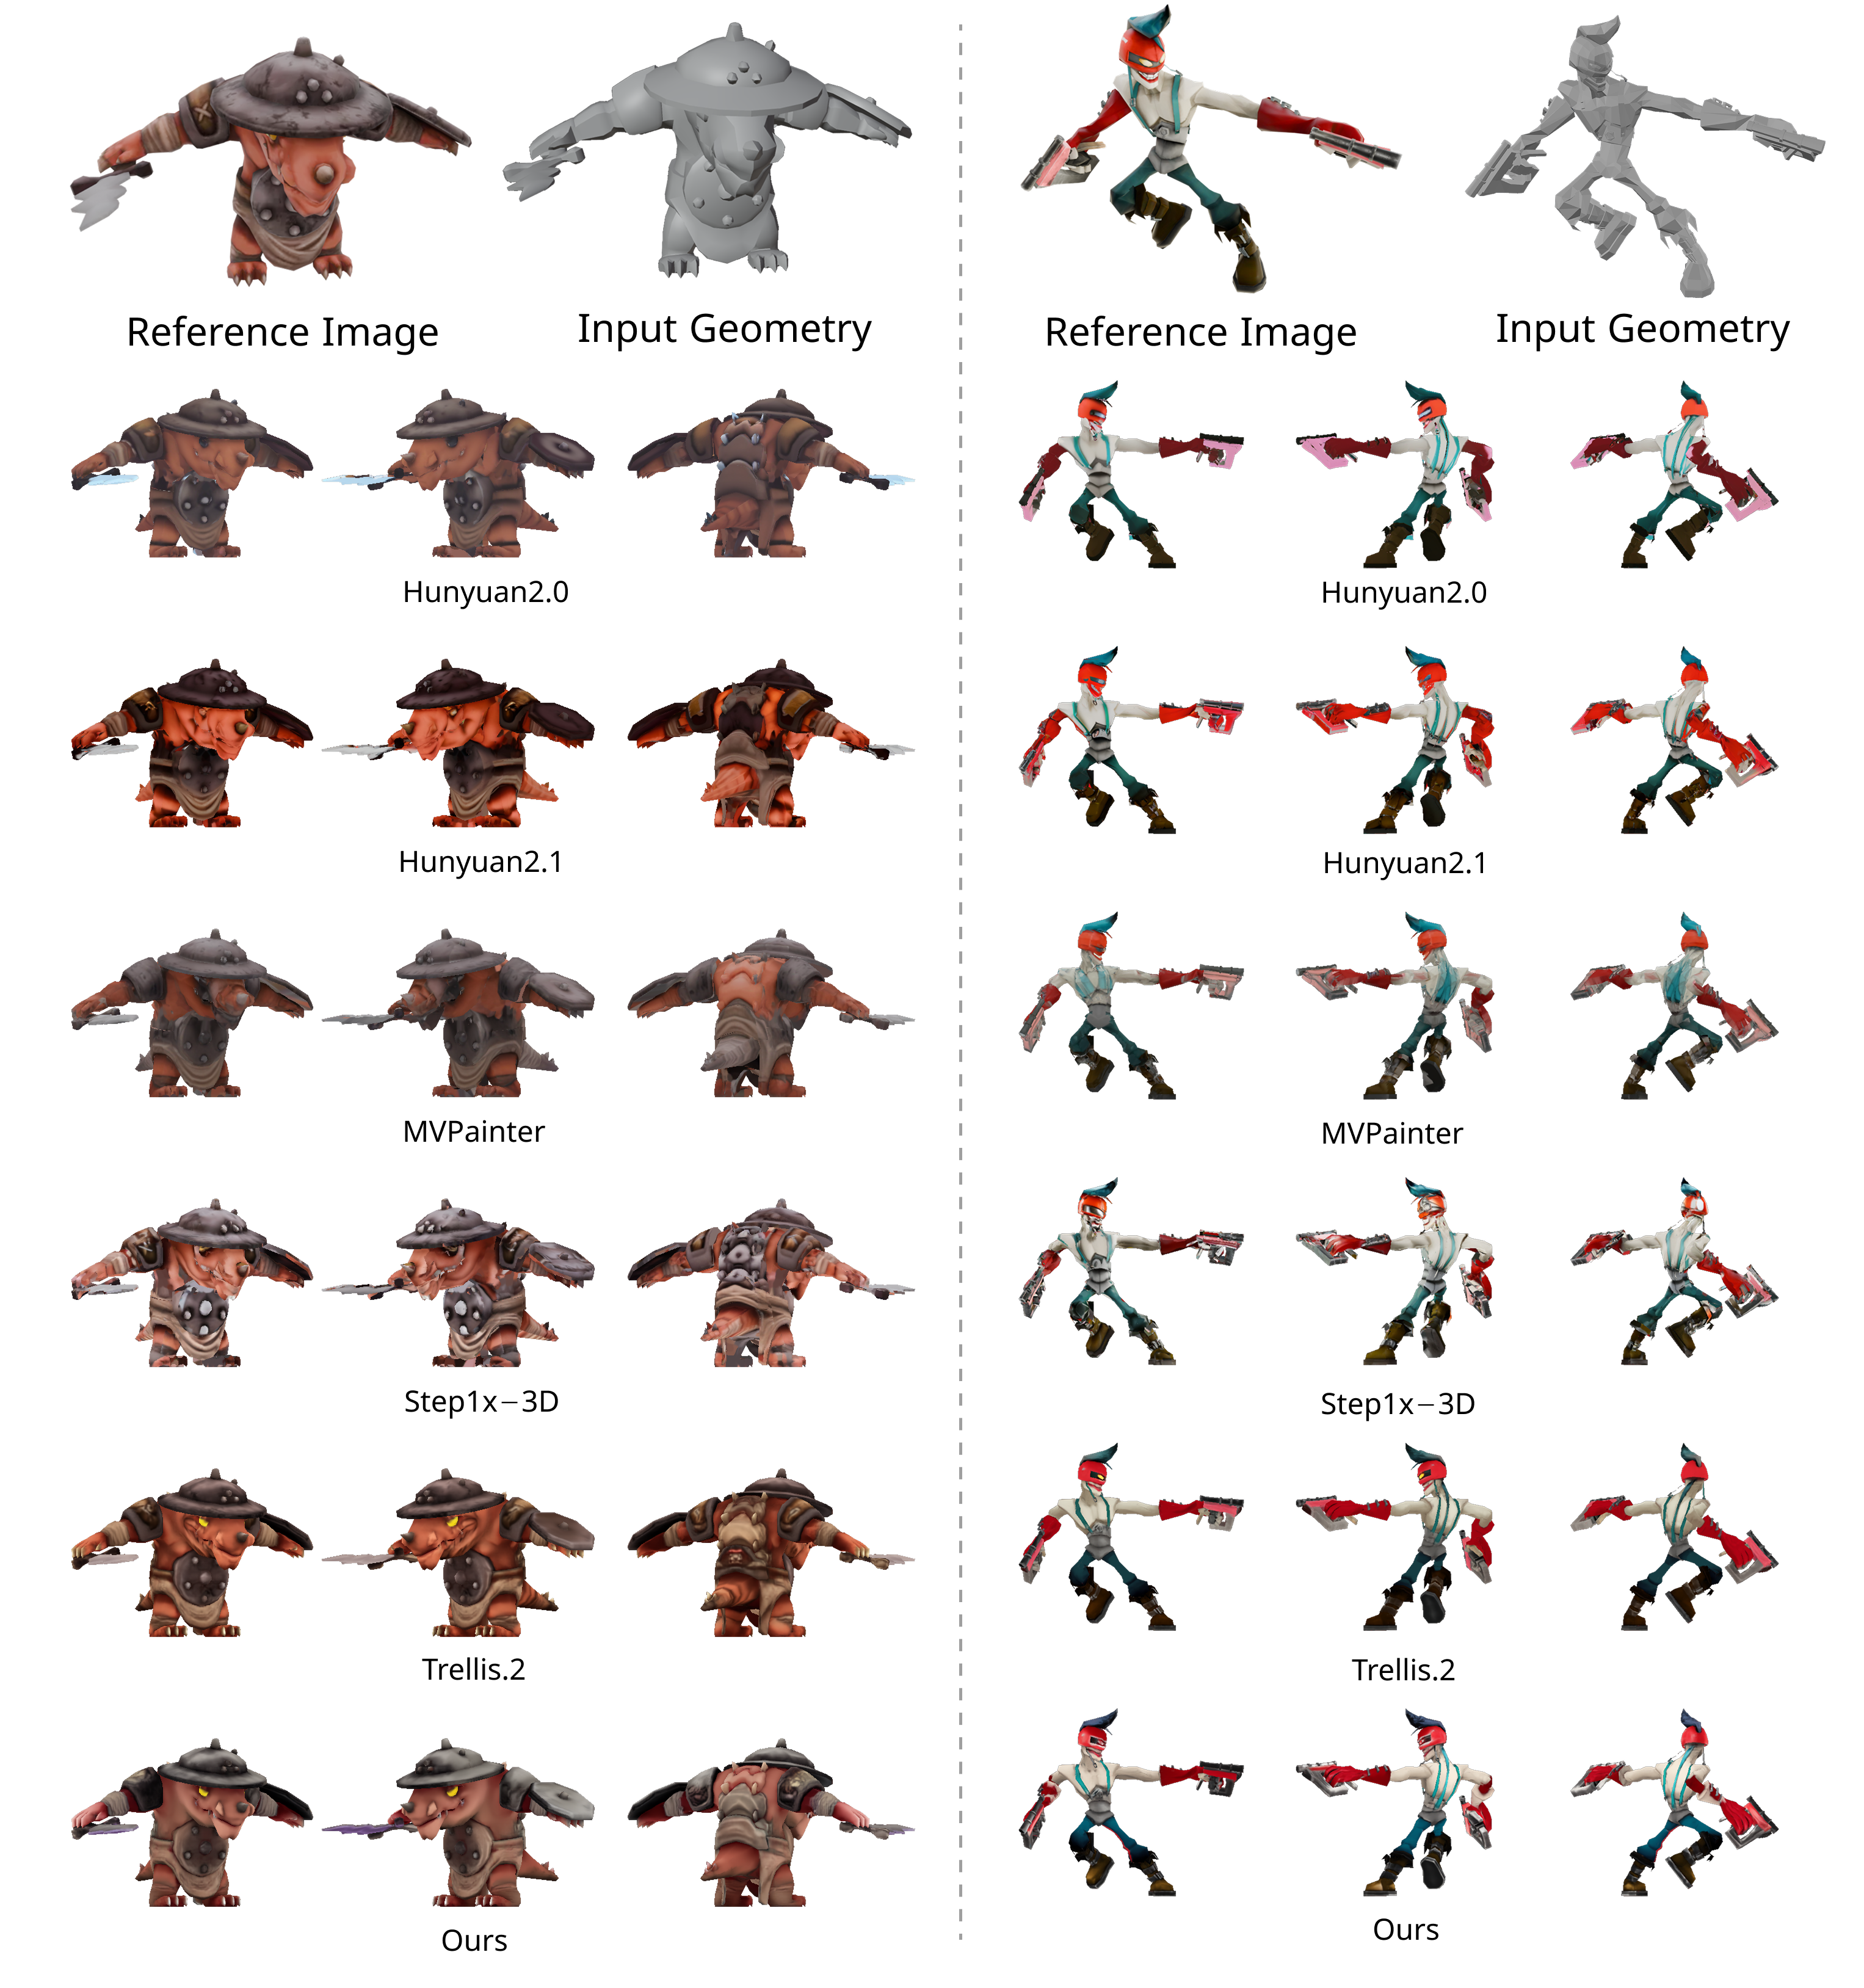
\includegraphics[width=\textwidth]{figure/final/qualitative_compare.png}
    \caption{
    纹理生成定性对比结果。
    每列分别展示不同方法生成结果在多个视角下的渲染效果。
    第一行为参考图像与对应裸网格，
    后续各行为不同方法生成的纹理结果。
    可以观察到，本文方法在保持正面纹理细节的同时，
    能够生成更加连贯、符合语义的侧面与背面纹理，
    整体视觉质量优于其他方法。
    }
    \label{fig:qualitative_compare}
\end{figure*}

从图~\ref{fig:qualitative_compare} 可以观察到，
多数基线方法能够在正面区域较好地复现参考图像中的主体颜色与局部纹理，
但在侧面与背面区域容易出现纹理模糊、
颜色不连续以及结构错位等问题。
特别是在角色背部与遮挡区域，
部分方法会生成明显的纹理拉伸、
随机颜色块或不符合语义的细节。

相比之下，
本文方法由于引入了多视角扩散生成的先验信息，
能够为三维纹理生成提供更加完整的视角约束，
因此在不可见区域的补全上表现更加稳定。
无论是怪物角色的大面积皮肤纹理，
还是人形角色的服饰边缘与武器细节，
本文方法均能够在不同视角之间保持较好的纹理连续性与语义一致性。
同时，
本文方法在背面区域生成了更加合理的颜色分布与结构细节，
有效减少了传统单视角驱动方法中常见的“正面清晰、背面失真”现象。

特别地，与未经微调、仅依赖单张参考图像驱动纹理生成的 Trellis.2 相比，
本文方法生成的纹理整体色调更加统一，更符合语义
在角色边缘区域的过渡也更加自然，
说明多视角先验不仅提升了局部细节保真度，
也增强了全局纹理分布的一致性。
该结果与前文定量实验中 FID 与 CMMD 指标的提升趋势一致，
进一步验证了本文方法在三维纹理生成任务中的有效性。